%! Author = zarnold
%! Date = 9/27/20

% Preamble
\documentclass[11pt]{article}
\usepackage{cite}
\usepackage{url}
\usepackage{fancyhdr}
% Packages
\usepackage{amsmath}
\usepackage{graphicx}
\usepackage[english]{babel}
\usepackage{lipsum}
\fancypagestyle{firstpage}
{
\fancyhead[L]{}
\fancyhead[R]{Zach Arnold \linebreak CS 7641 \linebreak Assignment 2}
\setlength{\headheight}{52pt}
}
\graphicspath{./}
\newcommand{\problemone}{One Max Problem}
\newcommand{\problemtwo}{K Color Problem}
\newcommand{\problemthree}{Some other problem}
% Document
\begin{document}
    \thispagestyle{firstpage}


    \section{Introduction}
    In this paper I will be exploring the performance and trade-offs of four randomized optimization algorithms: randomized hill climbing,
    simulated annealing, genetic algorithms, and MIMIC against three problems.
    Later in the paper I will rexamine work I did previously in Assigment 1 and attempt to optimize the weights of a multi-layered perceptron using these same
    four algorithms.
    For the purposes of this assignment I used the mlrose library\cite{Hayes19} which was publicly available.


    \section{Comparison of Randomized Optimization Algorithms}
    This section is dedicated to a comparison of the four algorithms andomized hill climbing,
    simulated annealing, genetic algorithms, and MIMIC against the \problemone.
    I will briefly introduce parameters I will be varying for each algorithm here and then we will compare their performance
    in each problems subsection below.
    \subsubsection*{Simulated Annealing}
    Simulated Annealing
    \subsubsection*{Randomized Hill Climbing}
    \subsubsection*{Genetic Algorithm}
    \subsubsection*{MIMIC}

    \subsection{\problemone}
    The \problemone is a fitness function that seeks to maximize a vector $v$ such that:
    \begin{equation}
        \label{oneMax}
        \sum_{i=0}^{n-1} v_i
    \end{equation}
    is a maximum, where $v_i$ is the $i$th component of vector $v$ with length $n$.
    This is a relatively easy optimization problem to understand and it illustrates the effectiveness of MIMIC and Genetic Algorithms
    quite nicely from an efficiency standpoint.
    \linebreak
    \begin{figure}
        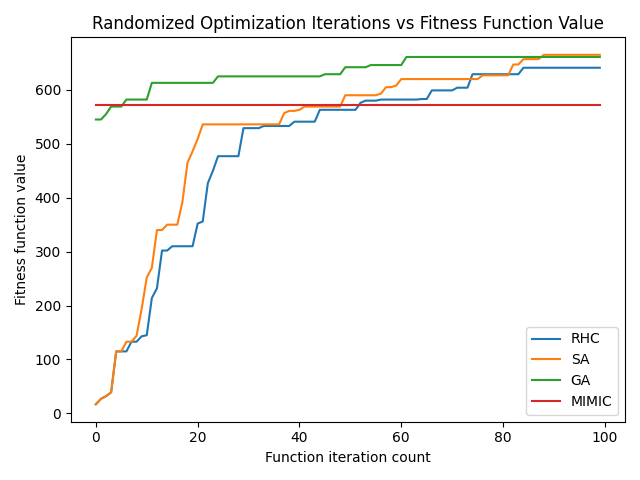
\includegraphics[scale=0.5]{onemax.png}\label{fig:oneMax}
    \end{figure}

    \subsection{8-Queens}
    The eight queens problem is a specific implementation of the n-queens optimization problem.\cite{Russel10} It poses
    an $n x n$ board like in chess where $n$ queens need to be placed such that a minimum number of queens could "attack"
    each other (diagonally, horizontally, or vertically.)
    \linebreak
    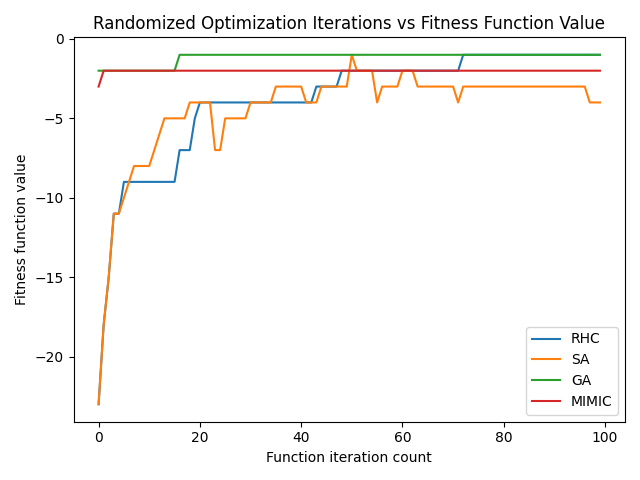
\includegraphics[scale=0.5]{eightqueens.png}

    \subsection{K-Colors}


    \section{Neural Network Weight Optimization}
    \bibliography{assignment2}{}
    \bibliographystyle{plain}
\end{document}